% Lecture file created by Gemini
% Class: Quantum Information With Atoms and Photons
% Professor: Pietro Silvi
% Date: 2025-10-16
\lecture{4}{Alkali and dipole selection rules}{2025-10-16}

% --- Start writing here ---
\captionsetup{singlelinecheck=false}
Atoms of Group I From Hydrogen to Alkall\\
$\rightarrow$ THREE LEVELS OF DEPTM (PERTURBATION SPLIT)\\
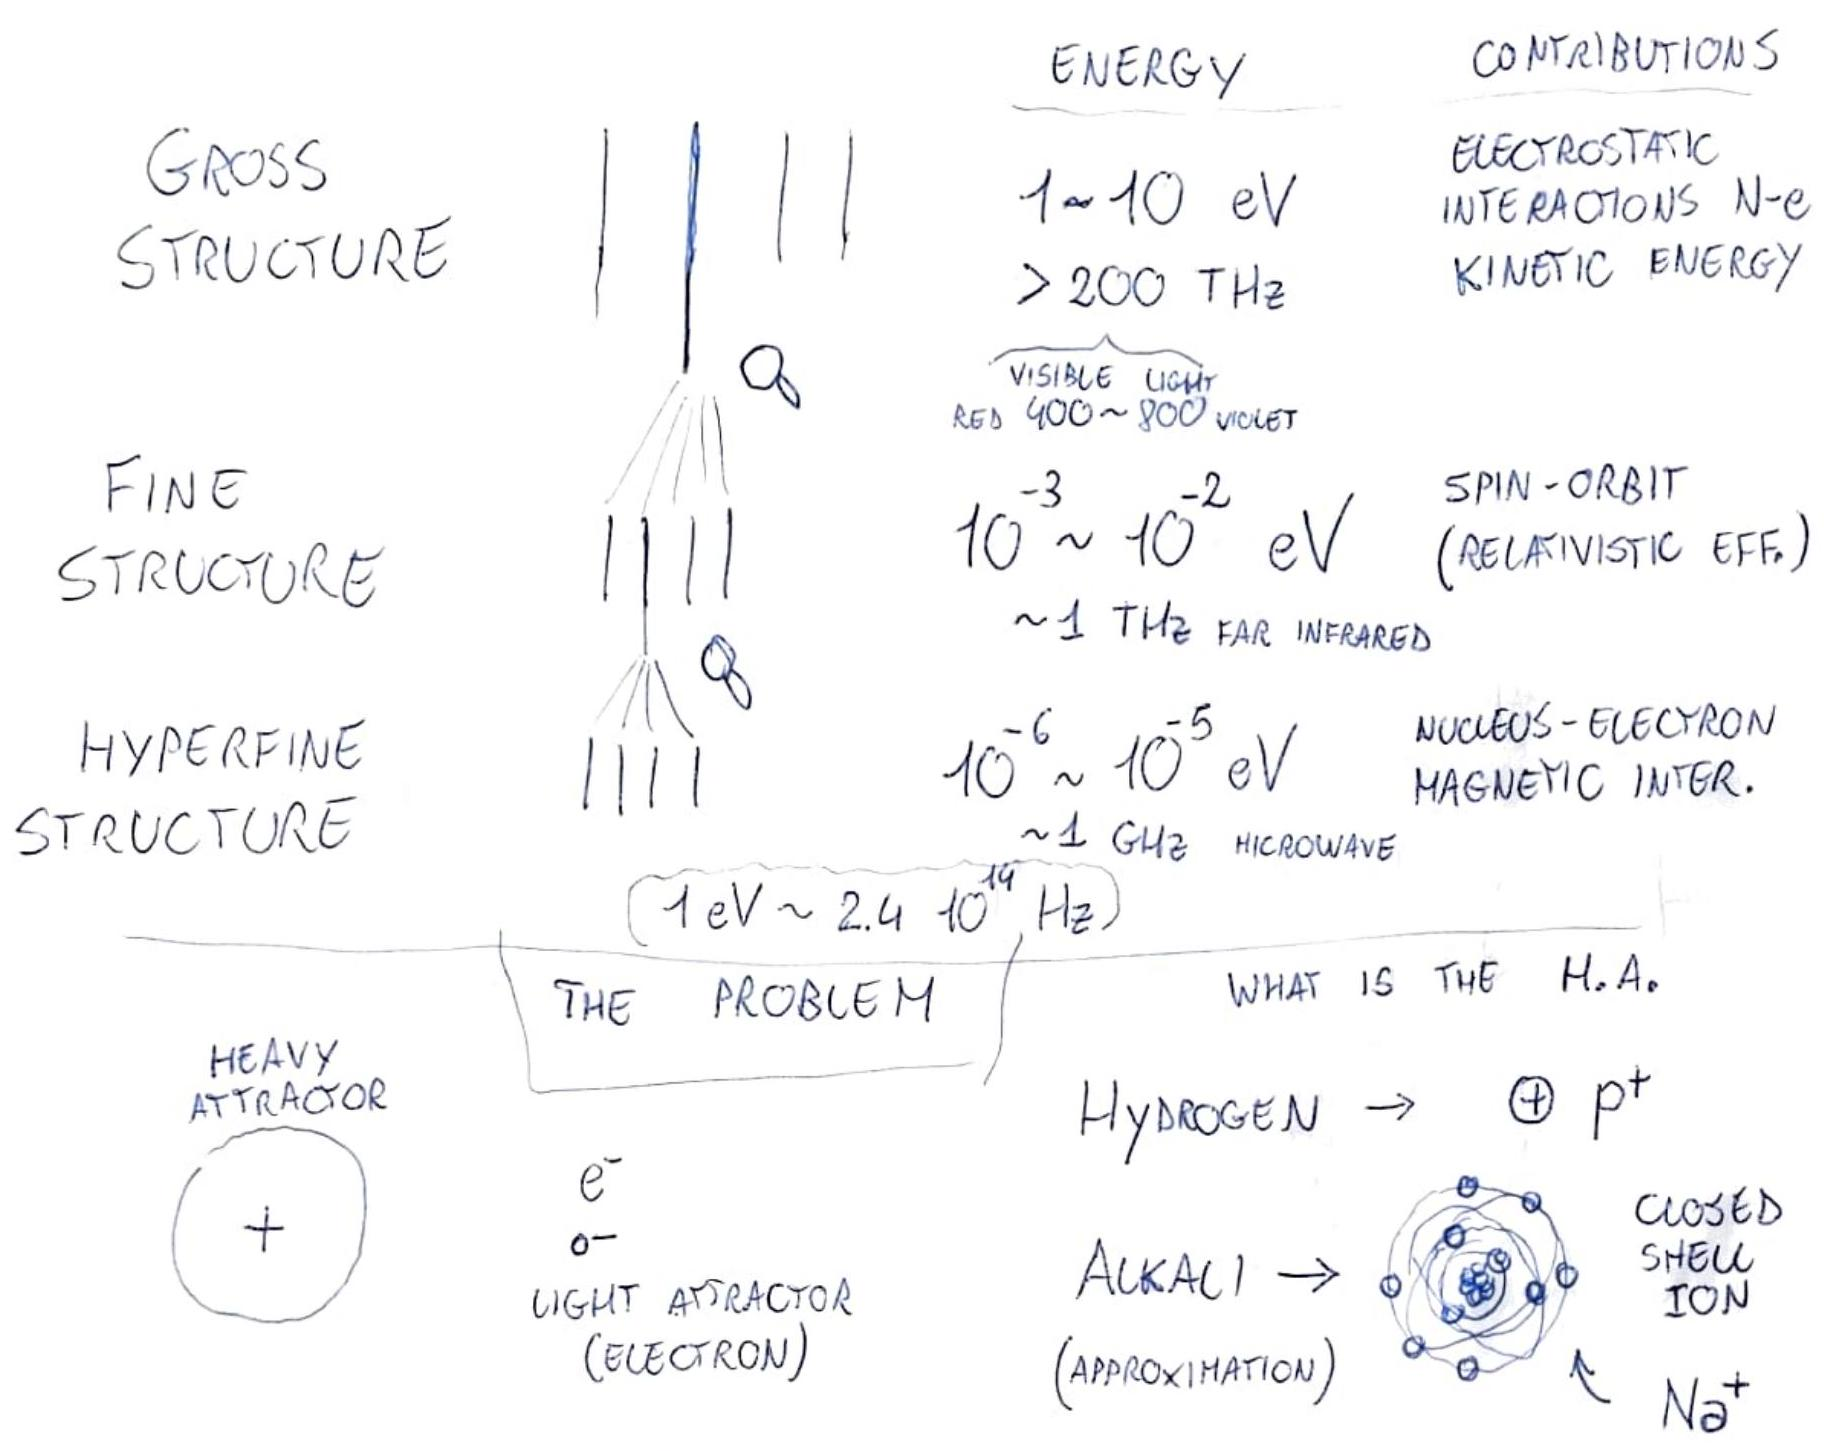
\includegraphics[max width=\textwidth, center]{2025_10_16_22329e0f50bdd2511b17g-01}

Effective 2-BODY Dynamics:

$$
H=\underbrace{\frac{\left|\vec{p}_{H}\right|^{2}}{2 m_{H}}}_{\substack{\text { HEAYY KINETIC } \\ \text { (NON RELATIVISTIC) }}}+\underbrace{\frac{\left|\vec{p}_{e}\right|^{2}}{2 m_{e}}}_{\substack{\text { ELECTRON KINETK } \\ \text { (SOMEHON STILU } \\ \text { NON RELATIVISTIC }}}+\overbrace{V\left(\left|\vec{r}_{H}-\vec{r}_{e}\right|\right)}
$$

Step 1 change of coorsinates

$$
\begin{gathered}
\text { CENTER-OF-MASS } \\
\text { COORDINATE } \\
\text { AND HOMENTUM }
\end{gathered}
$$

$$
\vec{R}=\frac{\vec{r}_{e} m_{e}+\vec{r}_{H} m_{H}}{m_{e}+m_{H}} \quad \vec{P}=\vec{P}_{e}+\vec{P}_{H}
$$

$$
\begin{aligned}
& \text { RELATIVE } \\
& \text { COORDINATE } \\
& \text { AND MOMENTUM }
\end{aligned}
$$

$$
\vec{r}=\vec{r}_{e}-\vec{r}_{H} \quad \vec{p}=\frac{\frac{\vec{p}_{e}}{m_{e}}-\frac{\vec{p}_{H}}{m_{H}}}{\frac{1}{m_{E}}+\frac{1}{m_{H}}}
$$

$$
\begin{gathered}
{\left[r_{e}, p_{e}\right]=i \hbar} \\
{\left[r_{H}, p_{H}\right]=i \hbar} \\
{\left[r_{e}, p_{H}\right]=\left[r_{H}, p_{e}\right]=0}
\end{gathered} \quad \backsim \quad\left[\begin{array}{l}
{[R, P]=[r, P]=i \hbar} \\
{[R, P]=[r, P]=0}
\end{array}\right.
$$

$$
m_{t}=m_{e}+m_{H} \approx m_{H}
$$

Where TOTAL HASS

$$
\begin{array}{r}
\frac{1}{m^{2}}=\frac{1}{m_{e}}+\frac{1}{m_{H}} \approx \frac{1}{m_{e}} \\
\text { RESUCES HASS }
\end{array}
$$

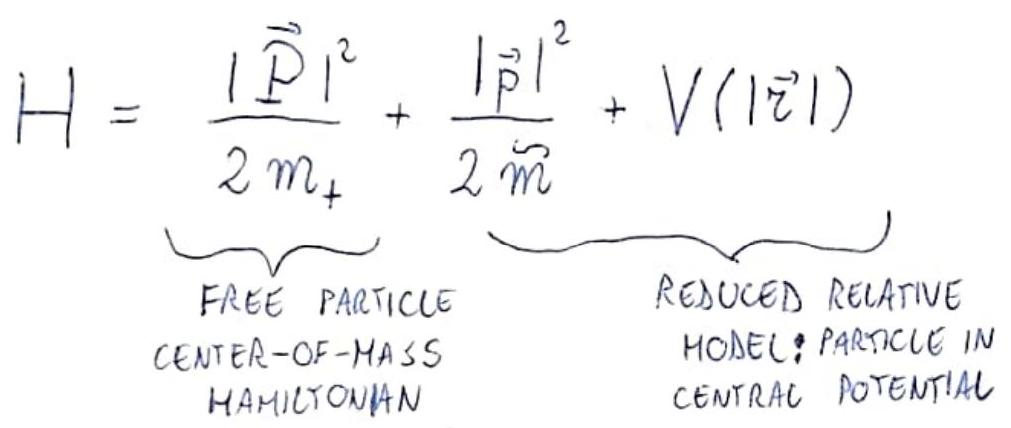
\includegraphics[max width=\textwidth]{2025_10_16_22329e0f50bdd2511b17g-02} $\binom{\text { but not helways }}{\text { refe! Recolu }} \longleftrightarrow$ we can ignore this part for now

$$
\begin{aligned}
& \frac{|\vec{p}|^{2}}{2 \vec{m}}=\left(\begin{array}{c}
\text { CARTESIAN } \\
\text { COORDINES } \\
x, y, z
\end{array}\right) \cdot \frac{-\hbar^{2}}{2 \vec{m}}\left(\frac{\partial^{2}}{\partial x^{2}}+\frac{\partial^{2}}{\partial y^{2}}+\frac{\partial^{2}}{\partial z^{2}}\right) \\
& \text { EASY TO } \\
& \text { REMEMBER } \\
& = \\
& -\frac{\hbar^{2}}{2 m} \nabla^{2}\left(\begin{array}{c}
\text { POLAR } \\
\text { CORDMATES } \\
r, \theta, \varphi
\end{array}\right)-\frac{\hbar^{2}}{2 m}\left(\frac{1}{r^{2}} \frac{\partial}{\partial r}\left(r^{2} \frac{\partial}{\partial r}\right)+\frac{1}{r^{2} \sin \theta} \frac{\partial}{\partial \theta}\left(\sin \theta \frac{\partial}{\partial \theta}\right)+\frac{1}{r^{2} \sin ^{2} \theta} \frac{\partial^{2}}{\partial \varphi^{2}}\right) \\
& =-\frac{\hbar^{2}}{2 m}\left(\frac{1}{r^{2}} \frac{\partial}{\partial r}\left(r^{2} \frac{\partial}{\partial r}\right)\right)+\frac{1}{2 m r^{2}} L^{2} \\
& \text { 正 } \\
& \text { angular momentum. } \\
& \text { We nees a refresher }
\end{aligned}
$$

\section*{Orbital angular Momentum}
of a canchical pairi coor $\vec{r}$ inate $+\underset{\vec{p}}{\text { homentum }}$(lhe resuces (ones in this case)\\
reads $\vec{L}=\underbrace{\vec{r} \times \vec{p}}_{\substack{\text { VECTCR CROSS } \\ \text { PROSUCT }}} \quad \begin{gathered}\text { CIASSICAL-OR-} \\ \text { QUANUMAMCS } \\ \text { HECHANICS }\end{gathered}$\\
COHMUTE THUS ALSO\\
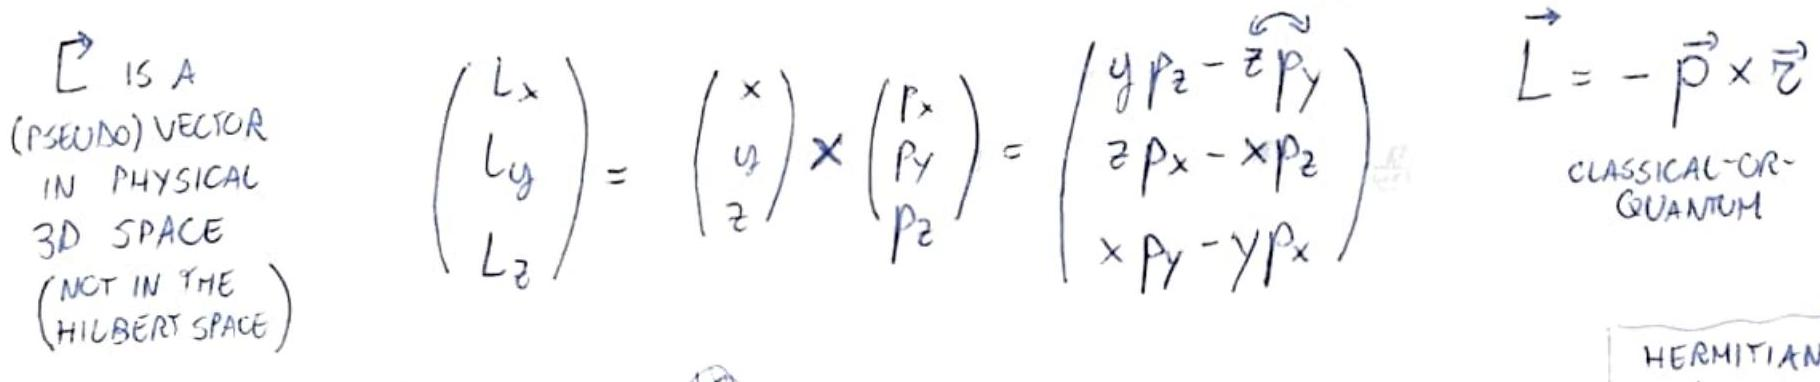
\includegraphics[max width=\textwidth, center]{2025_10_16_22329e0f50bdd2511b17g-03}

\section*{QUANTUM}
$\vec{r}$ and $\vec{P}$ are vectors $\quad L_{z}=-i \hbar\left(x \frac{\partial}{\partial y}-y \frac{\partial}{\partial x}\right)$ ete... OF OPERATORS,THLS\\
$\vec{L}$ as we U\\
$\vec{r}$ and $\vec{p}$ do not commute $D>L_{x}, L_{y}, L_{z}$ do not commute as well

$$
\begin{aligned}
& {\left[L_{x}, L_{y}\right]=-\hbar^{2}\left(\left(y \frac{\partial}{\partial z}-z \frac{\partial}{\partial y}\right)\left(z \frac{\partial}{\partial x}-x \frac{\partial}{\partial z}\right)-\left(z \frac{\partial}{\partial x}-x \frac{\partial}{\partial z}\right)\left(y \frac{\partial}{\partial z}-z \frac{\partial}{\partial y}\right)\right)} \\
& =-\hbar^{2}\left(y \frac{\partial}{\partial x}+y z \frac{\partial^{2}}{\partial z \partial x}-z^{2} \frac{\partial^{2}}{\partial x \partial y}-x y \frac{\partial^{2}}{\partial z^{2}}+x z \frac{\partial^{2}}{\partial y \partial z}\right)+ \\
& +\hbar^{2}\left(y z \frac{\partial^{2}}{\partial x \partial z}+x \frac{\partial}{\partial y}-x y \frac{\partial^{2}}{\partial z^{2}}-z^{2} \frac{\partial^{2}}{\partial x \partial y}+x z \frac{\partial^{2}}{\partial z \partial y}\right)= \\
& =\hbar^{2}\left(x \frac{\partial}{\partial y}-y \frac{\partial}{\partial x}\right)=i \hbar\left(x p_{y}-y p_{x}\right)=i \hbar L_{z} \text { AND BY EXTENGION } \\
& {\left[L_{i}, L_{j}\right]=i \hbar \underbrace{\varepsilon_{i jk}} L_{k}} \\
& \text { COMPUETECY ANTISYMMETRIC } \\
& \text { TENSOR } \\
& \text { TOTAL Angular } L^{2}=L_{x}^{2}+L_{y}^{2}+L_{z}^{2} \\
& \stackrel{\downarrow}{\text { commutes }}\left[L^{2}, L_{j}\right]=0 \quad \begin{array}{l}
\text { QUADRATIC } \\
\text { CASIMIR or. }
\end{array} \\
& \text { 《集 Closes lie Algebra } \\
& \text { OF HERMITIAN OPS. } \\
& \text { they generate continuous } \\
& \text { GROUPS (OF ROTATIONS) }
\end{aligned}
$$

EXAMPLE $\left[l^{2}, l_{z}\right]=\left[l_{x}^{2}, l_{z}\right]+\left[l_{y}^{2}, l_{z}\right]=$

$$
\begin{aligned}
& L_{x}^{2} L_{z}-L_{z} L_{x}^{2}+L_{y}^{2} L_{z}-L_{z} L_{y}^{2}= \\
& L_{x} L_{z} L_{x}+L_{x}\left[L_{x} L_{z}\right]-L_{x} L_{z} L_{x}-\left[L_{z} L_{x}\right] L_{x}+\ldots . .= \\
& \quad L_{x}\left(-i L_{y}\right)-\left(i L_{g}\right) L_{x}+L_{y}\left(+i L_{x}\right)-\left(-i L_{x}\right) L_{y}=0
\end{aligned}
$$

$\underset{\substack{\text { RAISING AND } \\ \text { COWERING }}}{\text { OPERATORS }}\left\{\begin{array}{l}L_{ \pm}=L_{x} \pm i L_{y} \leftarrow \text { NOT HERMITIAN }\left(L_{+}\right)^{+}=L_{x}^{+}+(i)^{*} L_{y}^{+}=L_{-} \\ {\left[L_{+}, L_{-}\right]=i\left[L_{y}, L_{x}\right]-i\left[L_{x}, L_{y}\right]=2 \hbar L_{z}} \\ {[1,1]}\end{array}\right.$

$$
\begin{aligned}
{\left[L_{z}, L_{ \pm}\right] } & =\left[L_{z}, L_{x}\right] \pm i\left[L_{z}, L_{y}\right]= \\
& =i \hbar L_{y} \pm \hbar L_{x}= \pm \hbar\left(L_{x} \pm i L_{y}\right)= \pm \hbar L_{ \pm}
\end{aligned}
$$

$$
\begin{aligned}
L^{2} & =L_{x}^{2}+L_{y}^{2}+L_{z}^{2} \\
& =L_{-} L_{+}+L_{z}^{2}+\hbar L_{z} \\
& =L_{+} L_{-}+L_{z}^{2}-\hbar L_{z}
\end{aligned}
$$

alternative ways OF WRITING $L^{2}$\\
heaning of labels\\
$\left[L^{2}, L_{z}\right]=0 \sim \underset{\substack{\text { SIMULTANEOUS } \\ \text { WAVERUCTION }}}{\text { EIGNG }} \psi(l, m) \quad\left\{\begin{array}{l}L_{z} \psi(l, m)=\hbar m \psi \\ L^{2} \psi(l, m)=f(l) \psi\end{array}\right.$\\
ACTION OL THE\\
$\begin{aligned} & \text { ACTION OF THE } \\ & \text { RAISING /LOWERING ? } \\ & \text { OPERATOR }\end{aligned} ? L_{ \pm} \psi(e, m)>$

\section*{TWO OPTIONS}
$$
\begin{aligned}
& L^{2}\left(L_{ \pm} \psi(e, m)\right)=f(e)\left(L_{ \pm} \psi(e, m)\right) \\
& L_{z}\left(L_{ \pm} \psi(e, m)\right)= \\
& L_{ \pm} L_{z} \psi+\left[L_{z}, L_{ \pm}\right] \psi= \\
& \hbar m\left(L_{ \pm} \psi\right) \pm \hbar\left(L_{ \pm} \psi\right)=\hbar(m \pm 1) \psi
\end{aligned}
$$

(1) $L_{+} \psi(e, m) \propto \psi^{\prime}(e, m+1)$\\
(2) $L_{+} \psi(l, m)=0$\\
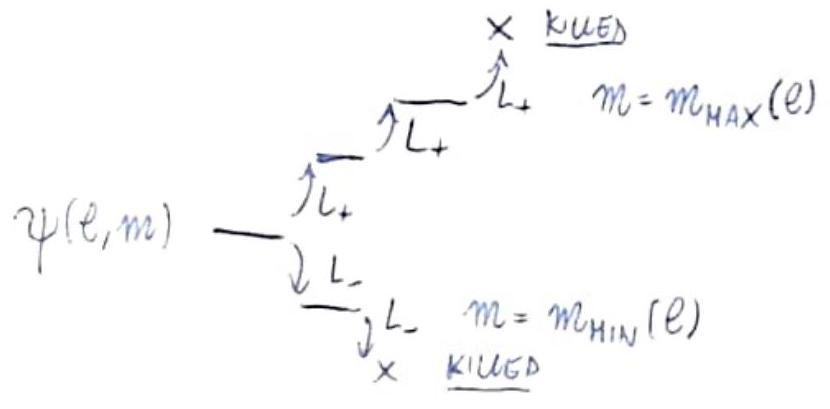
\includegraphics[max width=\textwidth, center]{2025_10_16_22329e0f50bdd2511b17g-04}\\
$L+\psi\left(e, m_{\text {HAX }}(e)\right)=0$ BUT\\
$L^{2}=\psi\left(l, m_{\text {HAX }}\right)=\left(L-L_{+}+L_{z}^{2}+\hbar L_{z}\right) \psi$\\
$f(e) \psi\left(e, m_{\text {HAX }}\right)=L_{x} \psi+L_{2}^{2} \psi\left(e, m_{\text {HAX }}\right)+\hbar L_{z} \psi\left(e, m_{\text {HAX }}\right)$

$$
\begin{aligned}
& =\left(\hbar^{2} m_{\text {HAX }}^{2}+\hbar^{2} m_{\text {HAX }}\right) \psi \\
f(e) & =\hbar^{2} m_{\text {HAX }}(e)\left(1+m_{\text {HAX }}(e)\right) \sqrt{ } \operatorname{sinICARCY}
\end{aligned}
$$

$1-\psi\left(e, m_{\text {HIN }}\right)=0$\\
$f(e) \psi\left(e, m_{\text {HIN }}(e)\right)=L^{2} \psi=L_{+} L \gamma\left(l, m_{\text {H } N}\right)+L_{2}^{2} \psi-\hbar L_{z}=\hbar^{2}\left(m_{\text {H } N}-i\right) m_{\text {M } N} \psi$

$$
f(e)=\hbar^{2} m_{\text {MIN }}\left(m_{\text {HIN }}-1\right)
$$

SYSTET $\left\{\begin{array}{l}m_{\text {HAX }}\left(m_{\text {HAX }}+1\right)=m_{\text {HIN }}\left(m_{\text {MIN }}-1\right) \\ m_{\text {MAX }}-m_{\text {MIN }}=\frac{\hbar}{\hbar} N\end{array}\right.$

\section*{SOUTTION}
$$
\left\{\begin{aligned}
m_{\text {HAX }}= & \begin{array}{r}
\text { POSITIVE INTEGER } \\
\text { TOS, HALF INTEGER }
\end{array} \\
m_{\text {HIN }}= & -m_{\text {MAX }}
\end{aligned}\right.
$$

FROM NOW EN, WE LABEL $l=m_{\text {HAX }}$

$$
\begin{aligned}
& L_{-}^{2} \psi(l, m)=\hbar^{2} l(l+1) \psi(l, m) \\
& L_{z} \psi(l, m)=\hbar m \psi(l, m)
\end{aligned}
$$

$$
f(e)=\hbar^{2} e(e+1)
$$

WHERE $l \in \frac{\mathbb{N}}{2}$ AND $\quad m \in\{-l, \ldots,+l\}$\\
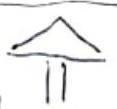
\includegraphics[width=0.5\textwidth, center]{2025_10_16_22329e0f50bdd2511b17g-05}

However, these ruces simply foulow from the algebra structure

$$
\left[A_{i}, A_{j}\right]=i \hbar \varepsilon_{i j k} A_{k}
$$

and use no other information. even the "internal hagentic bipole moment" (aka spin) obeys these rules.\\
4.T THE OrbITAL angular momentum has more structure\\
$\vec{L}=\vec{r} \times \vec{p}$ WHICH IMPOSES FURTHER RESTRICTIONS

\section*{TRICK}
$L_{z}=r_{x} p_{y}-r_{y} p_{x}$\\
$r_{1}^{2}-r_{2}^{2}=2 r_{x} p_{y}$\\
$p_{1}^{2}-p_{2}^{2}=-2 r_{y} p_{x}$\\
THUS\\
$L_{z}=\underbrace{\frac{1}{2}\left(r_{1}^{2}+p_{1}^{2}\right)}_{\substack{\text { GUANY } \\ \text { HANY. } \\ \text { OSCICT } \\ H_{1}}}-\underbrace{\frac{1}{2}\left(r_{2}^{2}+p_{2}^{2}\right)}_{\substack{\text { ANT } \\ \text { ONE }}}$\\
$\left[L_{z}, H_{1}\right]=\left[L_{z}, H_{2}\right]=0$

$$
\left[H_{1}, H_{2}\right]=0
$$

$$
L_{z}=H_{1}-H_{2} \quad \hbar m \psi=L_{z} \psi=\hbar\left(\left(n_{1}+\frac{1}{2}\right)-\left(n_{2}-\frac{1}{2}\right)\right) \psi
$$

$$
\left.\begin{array}{c}
m=n_{1}-n_{2} \\
\stackrel{\leftarrow}{\mathbb{Z}} \\
\stackrel{\vdots}{\in \mathbb{Z}}
\end{array}\right\} \quad m \in \mathbb{Z} \rightarrow e \text { INTEGER! }
$$

But oncy when $\vec{L}=\vec{r} \times \vec{p}$\\
is arbital is orbital

Why is This Important?\\
$\left.\operatorname{AS}_{\text {SALD }} \omega E\right) \rightarrow-\frac{\hbar^{2}}{2 m}\left(\frac{1}{r^{2} \sin \theta} \frac{\partial}{\partial \theta}\left(\sin \theta \frac{\partial}{\partial \theta}\right)+\frac{1}{r^{2} \sin ^{2} \theta} \frac{\partial^{2}}{\partial \varphi^{2}}\right)=\frac{|L|{ }^{2}}{2 m r^{2}}$\\
$H=\underbrace{-\frac{\hbar^{2}}{2 m}\left(\frac{1}{r^{2}} \frac{\partial}{\partial r}\left(r^{2} \frac{\partial}{\partial r}\right)\right)+V_{\text {CORE }}(r)}_{\text {OVY RADIAL }}+\frac{\left|L^{2}\right|}{2 m r^{2}}$

$$
\begin{gathered}
{\left[r, L^{2}\right]=\left[\frac{\partial}{\partial r}, L^{2}\right]=0} \\
\omega=0 \\
{\left[H, L^{2}\right]=0}
\end{gathered}
$$

\begin{center}
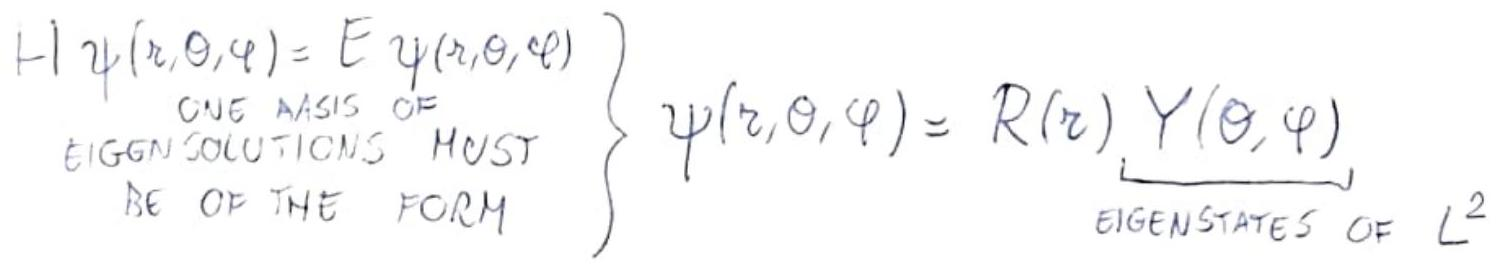
\includegraphics[width=0.5\textwidth]{2025_10_16_22329e0f50bdd2511b17g-06}
\end{center}

\section*{Angular Momentum un Polar Coordinates}
$(\hat{x}, \hat{y}, \hat{z}) \longrightarrow(\hat{r}, \hat{\theta}, \hat{\varphi})$\\
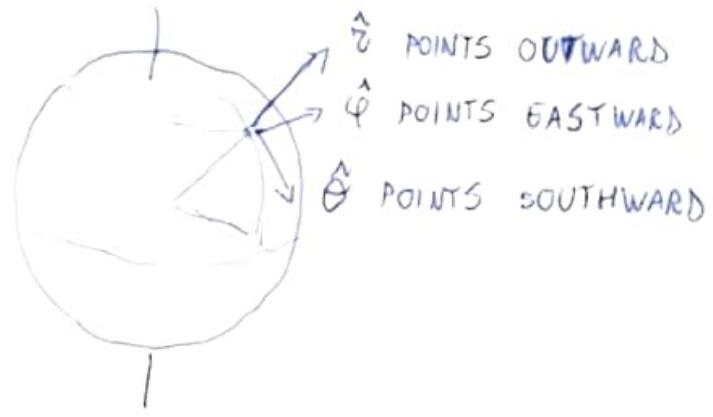
\includegraphics[width=0.5\textwidth, center]{2025_10_16_22329e0f50bdd2511b17g-07}

$$
\hat{r}=\left(\begin{array}{c}
\sin \theta \cos \varphi \\
\sin \theta \sin \varphi \\
\cos \theta
\end{array}\right) \quad \hat{\theta}=\left(\begin{array}{c}
\cos \theta \cos \varphi \\
\cos \theta \sin \varphi \\
-\sin \theta
\end{array}\right) \quad \hat{\varphi}=\left(\begin{array}{c}
-\sin \varphi \\
\cos \varphi \\
0
\end{array}\right)
$$

\section*{GRASIENT}
$$
\vec{\nabla}=\hat{r} \frac{\partial}{\partial r}+\hat{\theta} \frac{1}{r} \frac{\partial}{\partial \theta}+\hat{\varphi} \frac{1}{r \sin \theta} \frac{\partial}{\partial \varphi}
$$

$\left\{\begin{array}{c}\text { ANGULAR } \\ \text { MOMENTUM }\end{array}\right\} \vec{L}=\vec{r} \times \vec{p}=r \hat{r} \times(-i \hbar) \vec{\nabla}=$

$$
\begin{aligned}
& =-i \hbar\left(\hat{r} \times r^{2} r \frac{\partial}{\partial r}+\hat{r} \times \hat{\theta} r \frac{1}{r} \frac{\partial}{\partial \theta}+\hat{r} \times \hat{\varphi} \frac{r}{r \sin \theta} \frac{\partial}{\partial \varphi}\right) \\
\vec{L} & =-i \hbar\left(\hat{\varphi} \frac{\partial}{\partial \theta}-\hat{\theta} \frac{1}{\sin \theta} \frac{\partial}{\partial \varphi}\right)\left(\neq \begin{array}{c}
r \text { HAS } \triangle I S A P E C A R E D \\
\text { ANGULAR } \\
\text { ACTS ON ANGULES, ONC }
\end{array}\right.
\end{aligned}
$$

(EXAPPLE) $L_{z}=\hat{z} \cdot \vec{L}=-i \hbar\left(\hat{z} / \hat{\varphi} \frac{\partial}{\partial \theta}-\hat{z} \cdot \hat{\theta} \frac{1}{\sin \theta} \frac{\partial}{\partial \varphi}\right)=+i \hbar \frac{(-\sin \theta)}{\sin \theta} \frac{\partial}{\partial \varphi}$

$$
L_{z}=-i \hbar \frac{\partial}{\partial \varphi} \quad\left\{\begin{array}{l}
\varphi \rightarrow \text { ANGLE AROUND THE } z \text {-AXIS } \\
L_{z} \rightarrow \text { DERIVATIVE W/RESPECT TO } \varphi
\end{array}\right.
$$

$\xrightarrow{\text { NOTTKE }}$ STATES WITH $m=0$

STATES WITH几者0

$$
\underset{\text { CONSTNNT IN }}{Y(\theta, \varphi)}=\underset{0}{Y(\theta)} \rightarrow \frac{\partial}{\partial \varphi} Y(\theta)=0_{0}^{\nabla}
$$

$$
Y(\theta, \varphi)=\tilde{Y}(\theta) e^{i m \varphi} \rightarrow i \hbar \frac{\partial}{\partial \varphi} Y(\theta, \varphi)=\hbar m Y
$$

(SIMILARCIY) $L_{x}=-i \hbar(\overbrace{\hat{x} \cdot \hat{\varphi}}^{-\sin \varphi} \frac{\partial}{\partial \theta}-\overbrace{\hat{x} \cdot \hat{\theta}}^{\cos \theta \cos \varphi} \frac{1}{\sin \theta} \frac{\partial}{\partial \varphi})=$

$$
\begin{aligned}
& =i \hbar\left(\sin \varphi \frac{\partial}{\partial \theta}+\cot \theta \cos \varphi \frac{\partial}{\partial \varphi}\right) \\
L_{y} & =i \hbar\left(-\cos \varphi \frac{\partial}{\partial \theta}+\cot \theta \sin \varphi \frac{\partial}{\partial \varphi}\right)
\end{aligned}
$$

(AND THUS)


\begin{align*}
& L_{+}=L_{x}+i L_{y}=i \hbar\left(\cot \theta(\cos \varphi+i \sin \varphi) \frac{\partial}{\partial \varphi}+(\sin \varphi-i \cos \varphi) \frac{\partial}{\partial \theta}\right) \\
& =i \hbar\left(\cot \theta e^{i \varphi} \frac{\partial}{\partial \varphi}+(-i) e^{i \varphi} \frac{\partial}{\partial \theta}\right) \quad \text { ANACARCY FOR } L_{-} \\
& L_{ \pm}=i \hbar e^{ \pm i \varphi}\left(\cot \theta \frac{\partial}{\partial \varphi} \pm(-i) \frac{\partial}{\partial \theta}\right) \\
& L_{-} L_{+}=-\hbar^{2} e^{-i \varphi}\left(\cot \theta \frac{\partial}{\partial \varphi}+i \frac{\partial}{\partial \theta}\right) e^{i \varphi}\left(\cot \theta \frac{\partial}{\partial \varphi}-i \frac{\partial}{\partial \theta}\right)= \\
& \text { USING }\left(\left\{\frac{\partial}{\partial \varphi} e^{i \varphi}=e^{i \varphi}\left(i+\frac{\partial}{\partial \varphi}\right)\right)\right. \\
& =-\hbar^{2} e^{-i \varphi} e^{i \varphi}\left(\cot \theta\left(i+\frac{\partial}{\partial \varphi}\right)+i \frac{\partial}{\partial \theta}\right)\left(\cot \theta \frac{\partial}{\partial \varphi}-i \frac{\partial}{\partial \theta}\right)= \\
& =-\hbar^{2}\left[\cot ^{2} \theta\left(i \frac{\partial}{\partial \varphi}+\frac{\partial^{2}}{\partial \varphi^{2}}\right)+\cot \theta \frac{\partial}{\partial \theta}-i \cot \theta \frac{\partial^{2}}{\partial \theta \partial \varphi}+i \cot \theta \frac{\partial^{2}}{\partial \theta \partial \varphi}+\frac{\partial^{2}}{\partial \theta^{2}}\right. \\
& \text { USING 》) } \left.\frac{\mu}{\sin \theta} \frac{\partial}{\partial \theta}\left(\sin \theta \frac{\partial}{\partial \theta}\right)=\cot \theta \frac{\partial}{\partial \theta}+\frac{\partial^{2}}{\partial \theta^{2}}-\frac{i}{\sin ^{2}} \frac{\partial}{\partial \varphi}\right] \\
& L_{-} L_{+}=-\hbar^{2}\left[\frac{1}{\sin \theta} \frac{\partial}{\partial \theta}\left(\sin \theta \frac{\partial}{\partial \theta}\right)-i \frac{\partial}{\partial \varphi}+\cot ^{2} \theta \frac{\partial^{2}}{\partial \varphi^{2}}\right] \\
& |\vec{L}|^{2}=L_{-} L_{+}+L_{z}^{2}+\hbar L_{z}=(\downarrow)-\hbar^{2} \frac{\partial^{2}}{\partial \varphi^{2}}-i \hbar^{2} \frac{\partial}{\partial \varphi} \\
& L^{2}=-\hbar^{2}\left[\frac{1}{\sin \theta} \frac{\partial}{\partial \theta}\left(\sin \theta \frac{\partial}{\partial \theta}\right)+\frac{1}{\sin ^{2} \theta} \frac{\partial^{2}}{\partial \varphi^{2}}\right] \tag{$\omega$}
\end{align*}


$L_{+}|l, m\rangle=\alpha|l, m+1\rangle \quad$ BuT $\quad \beta=\langle l, m| L_{-}|l, m+1\rangle=\langle l, m+1| L_{+}|h l, m\rangle^{*}=\alpha^{*}$

$$
\begin{aligned}
L_{-} L_{+}|e, m\rangle= & |\alpha|^{2}|e, m\rangle=\left(L^{2}-L_{z}^{2}-\hbar L_{z}\right)|e, m\rangle=\left(e(e+1)-m^{2}-m\right) \hbar^{2}|e, m\rangle \\
& \alpha=\hbar \sqrt{e(e+1)-m(m+1)} e^{i \phi} Z_{\text {THIS PHASE CAN SE SET TO }} \text { ZERO }
\end{aligned}
$$

$\left[L^{2}, L_{z}\right]=0$ common eigengasis but $L_{z}$ acts only on $\varphi$

$$
\begin{aligned}
& L_{z} \psi(\theta, \varphi)=-i \hbar \frac{\partial}{\partial \varphi} \psi(\theta, \varphi) \rightarrow Y_{e, m}(\theta, \varphi)=\left.\tilde{Y}_{e m}(\theta) e^{i m \varphi} m \in\right|_{-e} ^{e} \\
& \psi_{e, m=e}(\theta, \varphi)=Y_{e, e}(\theta) e^{i \ell \varphi} \quad \underbrace{\substack{\text { max w } \\
m=e}} \\
& L+\psi_{e, e}=0 \nabla_{0}^{\nabla} \quad \hbar e^{i \varphi}\left(\frac{\partial}{\partial \theta}+i \cot \theta \frac{\partial}{\partial \varphi}\right) \widetilde{Y}_{e e}(\theta) e^{i e \varphi}=0 \\
& \left(\frac{\partial}{\partial \theta}+i \cot \theta\left(\frac{\partial}{\partial \varphi} e^{i e \varphi}\right)\right) \tilde{Y}_{e e}(\theta)=0 \\
& \theta \in[0, \pi] \\
& \text { Fi! Solution } \forall e l \\
& \mathrm{~N}_{0}, 4 \\
& e^{i \ell \varphi}\left(\frac{\partial}{\partial \theta}-e \cot \theta\right) \widetilde{Y}_{e e}(\theta)=0 \stackrel{\substack{\text { Differential } \\
\text { EQUATION } \\
\text { SOLUTION }}}{\tilde{Y}_{e e}(\theta) \propto \sin ^{l}(\theta)} \\
& \underset{\longrightarrow}{\text { Normalization }} \int e^{-i l \varphi} \sin ^{e} \theta e^{+i l \varphi} \sin ^{e} \theta(d \varphi \sin \theta d \theta)=2 \pi \int_{0}^{\pi} \sin ^{2l+1}(\theta) d \theta \\
& =2 \pi \int_{-1}^{1}(1-\mu)^{e} d \mu=\binom{\text { TRY } M A T}{\text { HOME }}=\frac{4 \pi 2^{2 e}(e!)^{2}}{(2 e+1)!} \\
& Y_{e e}(\theta, \varphi)=\underset{\substack{\text { CHOOSEA } \\
\text { PHASE }}}{(-1)^{e}}\left(\frac{(2 e+1)!}{4 \pi}\right)^{1 / 2} \frac{1}{2^{e} e!} \sin ^{e}(\theta) e^{i e \varphi} \\
& \left\{\begin{array}{ll}
\text { FIND THE } & \text { PHASE } \\
\text { OTHER } & \text { Ye, M }
\end{array} \quad L_{-}|e, m\rangle=\sqrt{\text { elet }+1 \text {-m(m-1) }}|e, m-1\rangle\right. \\
& Y_{e, m-1}=\frac{-\hbar e^{-i \phi}}{\sqrt{e(e+1)-m(m-1)}}\left(\frac{\partial}{\partial \theta}-i \cot \theta \frac{\partial}{\partial \varphi}\right) Y_{e, m}(\theta, \varphi)
\end{aligned}
$$

Spherical Hormonics

table of afew s.m.

$$
\left.Y_{0,0}(\theta, \varphi)=\sqrt{\frac{1}{4 \pi}} \quad\right\} \text { S orbital "SHAR p" }
$$

могинице $\quad \int\left|Y_{\text {ем }}(\theta, \varphi)\right|^{2} \sin \theta d \theta d \varphi=1$

P orbital\\
"PRINCIPAL" BRIGHTEST LINES in FIOMIC SPECTRA OF AUKACI "DIFFUSE"

D crbital wibe fine structure\\
$Y_{20}(\theta, \varphi)=\frac{1}{4} \sqrt{\frac{5}{\pi}}\left(3 \cos ^{2} \theta-1\right)$

$$
\begin{aligned}
& Y_{2-1}=\ldots \quad \sin \theta \cos \theta e^{-i \varphi} \\
& Y_{2-2}=\ldots \quad \sin ^{2} \theta e^{-2 i \varphi}
\end{aligned}
$$

The radial part

$$
\begin{aligned}
& \psi(r, \theta, \varphi)=R(r) Y_{\text {em }}(\theta, \varphi) \quad H \psi=E \psi \\
& \left.R(r)=\frac{\hbar^{2}}{2 m} \frac{1}{r^{2}} \frac{\partial}{\partial r}\left(r^{2} \frac{\partial}{\partial r}\right)+\left[V_{\text {core }}(r)+\frac{\hbar^{2} e(e+1)}{2 m r^{2}}\right]\right) R(r)=E R(r) \\
& \left.\left.=\frac{1}{r^{2}} \frac{\partial}{\partial r}\left(r^{2} \frac{\partial}{\partial r}\right) \frac{P(r)}{r}=\frac{1}{r^{2}} \frac{\partial}{\partial r}\left(r \frac{\partial P}{\partial r}-P\right)=\frac{1}{r^{2}}\left(\frac{\partial P}{\partial r}+r \frac{\partial P}{\partial r}-\frac{\partial^{2} P}{\partial r^{2}}\right)\right)=\frac{\partial P}{\partial r}\right)=\frac{1}{r} \frac{\partial^{2}}{\partial r^{2}} P
\end{aligned}
$$

$$
\begin{aligned}
& Y_{3 m} \rightarrow F \text { ORBITAL } \\
& \text { FEW CRAZY EXPERIMENTAUSTS } \\
& \text { GO BEYONS } \log \text { FOR SANITY } \\
& \text { REASONS. }
\end{aligned}
$$

"FOORTH" or "FUNDAMENTAL"\\
$H \psi=E \psi$ 鸟, radial kinetic

$$
\left(-\frac{\hbar^{2}}{2 m} \frac{\partial^{2}}{\partial r^{2}}+\operatorname{Veff}\right) P(r)=E P(r)
$$

where $V_{\text {eff }}=+\frac{\hbar e(e+1)}{2 m r^{2}}-\frac{\left(Z_{\text {eff }}\right) e^{2}}{4 \pi \varepsilon_{0} r}$\\
7 angular kinetic $\frac{L^{2}}{2 I}, I=m r^{2}$\\
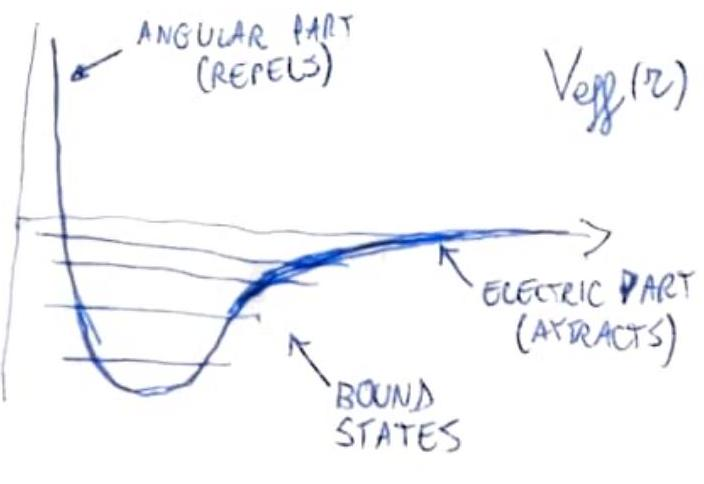
\includegraphics[width=0.5\textwidth, center]{2025_10_16_22329e0f50bdd2511b17g-11(1)}

SOLUTIONS CAN SEPENS ON I BUT NOT $m$

ACTUALUY\\
Hydrogen

\begin{figure}[h]
\begin{center}
\captionsetup{labelformat=empty}
\caption{Hydrogen}
  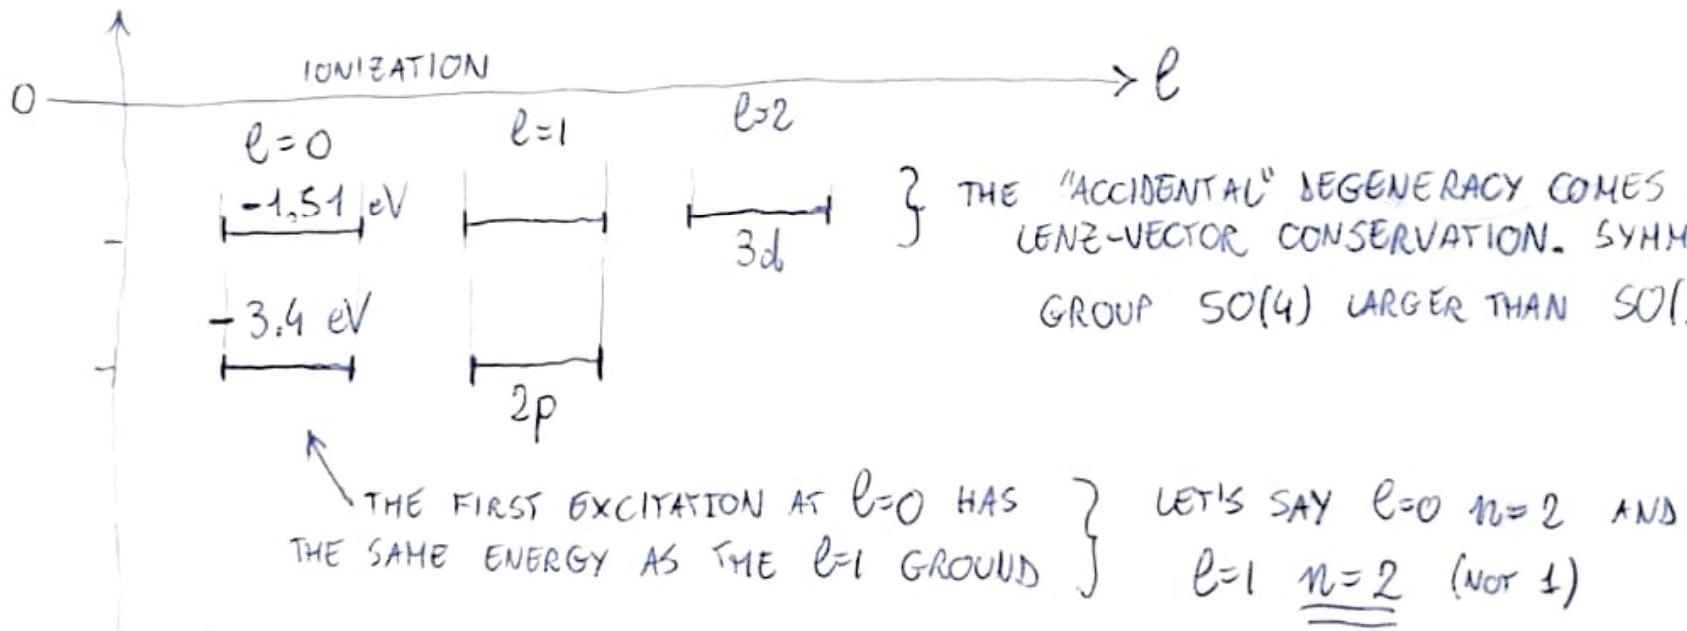
\includegraphics[width=\textwidth]{2025_10_16_22329e0f50bdd2511b17g-11(2)}
\end{center}
\end{figure}

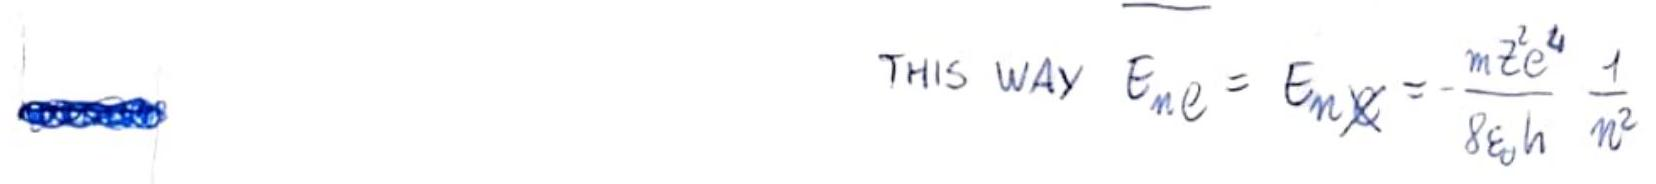
\includegraphics[width=0.5\textwidth, center]{2025_10_16_22329e0f50bdd2511b17g-11}\\
$\left.\frac{-13.6 \mathrm{eV}}{1 \mathrm{~s}} \leftarrow \begin{array}{l}\text { THE ground state } \\ \text { MAS } \quad l=0\end{array}\right\}$ LET'S say $n=1$\\
$\rightarrow$ In THIS NOTATION $l$ gues FROM 0 TO 1 - 1 ; BUT IT'S RATHER $\eta$ GOES FROM $C+1$ TO $\infty$, AND THE ENERGY DEPENDS ONLY ON $\eta$

Other alkall do not have the extra symmetay so the degeneracy is removes Eme, bot we use the same labeling conventons is removes Eme, but we use the same cabeling conventons

Ather Alkau - example: Sodum

$$
\begin{aligned}
H= & \sum_{j}^{\text {elec. }}\left(-\frac{\hbar^{2}}{2 m} \nabla_{j}^{2}-\frac{Z e^{2}}{4 \pi \varepsilon_{0} r_{j}}\right)+\sum \frac{e^{2}}{4 \pi \varepsilon_{0}\left|\vec{r}_{j}-\vec{r}_{j}\right|} \quad \text { Not SOUVABLE } \\
& \left.\frac{\text { GOOD APPROXIMATION }}{\text { HARTREE-FOCK }}\right\} \quad \begin{array}{l}
\text { NO CORRELATIONS/ENTANGLEMENT } \\
\rightarrow \text { ELEETIONG OCCUPY ORTHOGONAL ORBITALS } \\
\rightarrow \text { MINIMIZE ENERGY FUNCTIONAL OVER ORBITALS }
\end{array}
\end{aligned}
$$

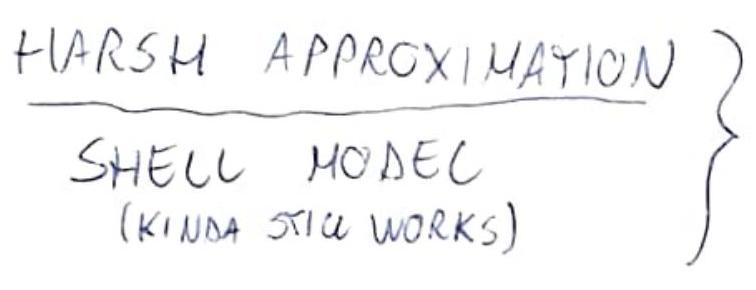
\includegraphics[width=0.5\textwidth, center]{2025_10_16_22329e0f50bdd2511b17g-12(2)}\\
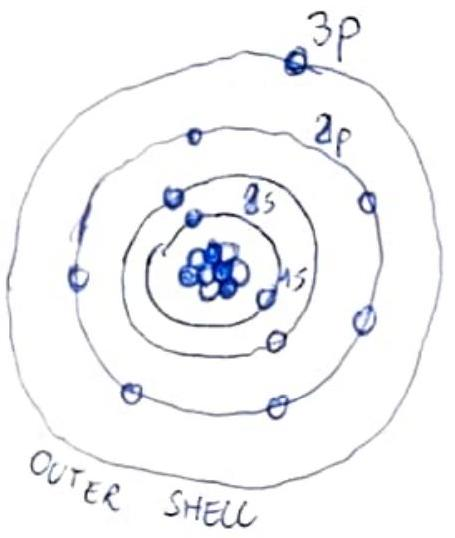
\includegraphics[width=0.5\textwidth, center]{2025_10_16_22329e0f50bdd2511b17g-12(1)}\\
$\rightarrow$ First, ELECTRONS FIU AN ATOMIC SHELL ( 2 (e+1) electrons in an eorsital)\\
$\rightarrow$ THEN, THEY SCREEN THE POETENTIAC\\
$\rightarrow$ REPEAT UNTIL NO MORE ELECTRONS

COTER SHELL EXPERIENCES \~{}HYDROGEN BUT MORE ATYRACTVE ccose to the core\\
\~{}HIGHER e PUSH e- ANNAY FROM THE CORE $\rightarrow$ LESS SHIFT\\
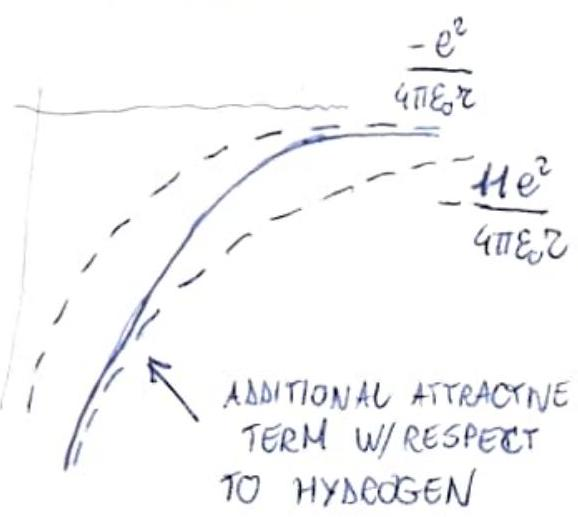
\includegraphics[width=0.5\textwidth, center]{2025_10_16_22329e0f50bdd2511b17g-12(3)}\\
thus, the 11th-electron of sodium sees the core as "acmost" a hydrogen, but not quite\\
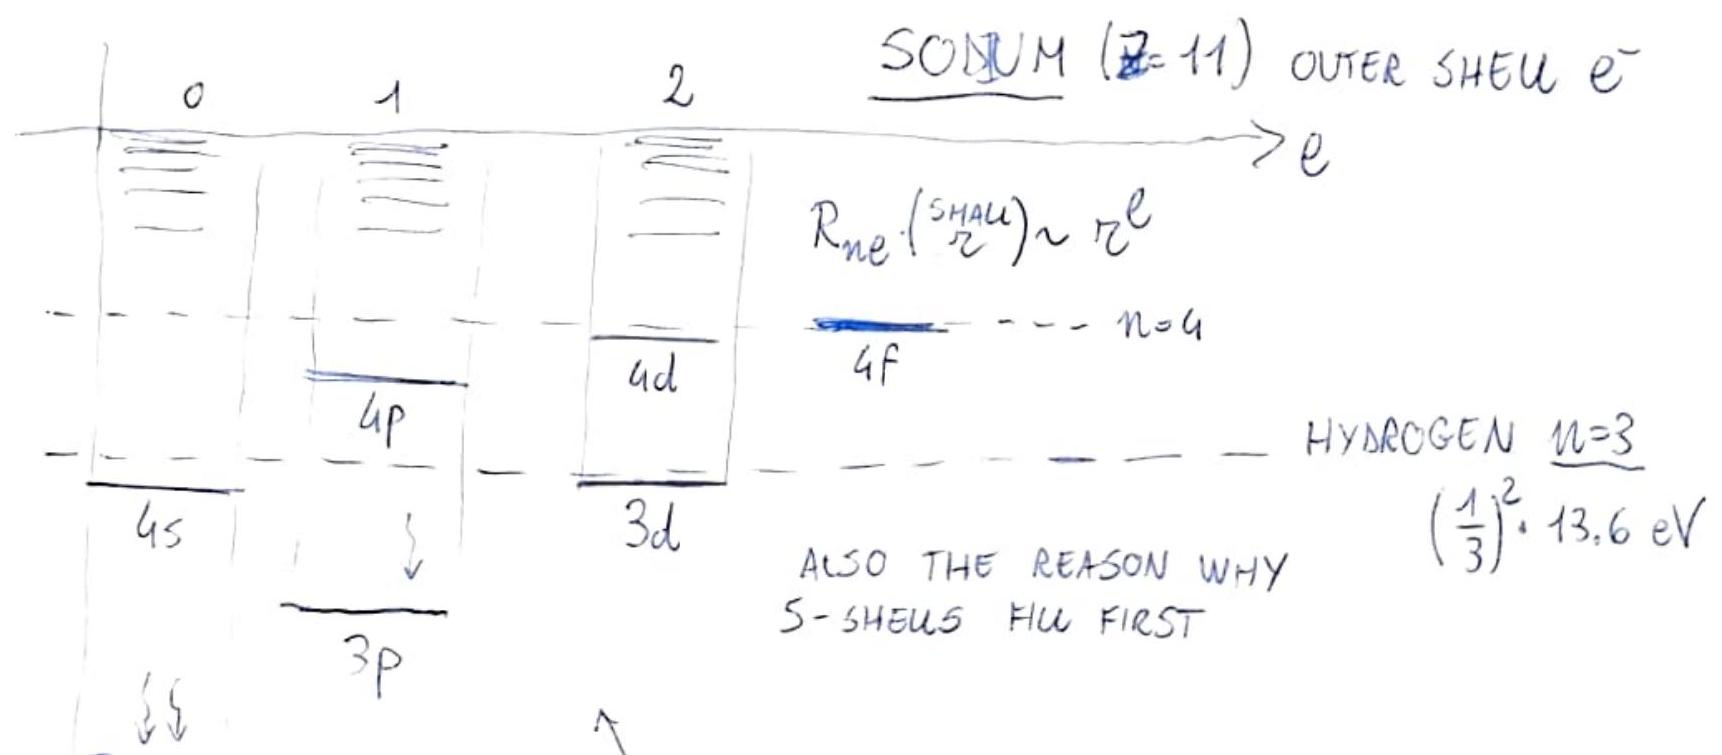
\includegraphics[width=0.5\textwidth, center]{2025_10_16_22329e0f50bdd2511b17g-12(4)}\\
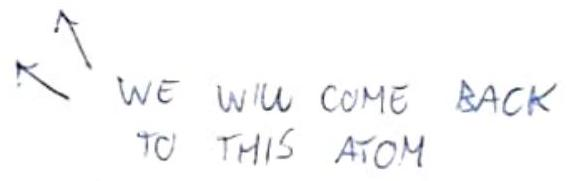
\includegraphics[width=0.5\textwidth, center]{2025_10_16_22329e0f50bdd2511b17g-12}

\section*{Dipole Transitions}
\begin{center}
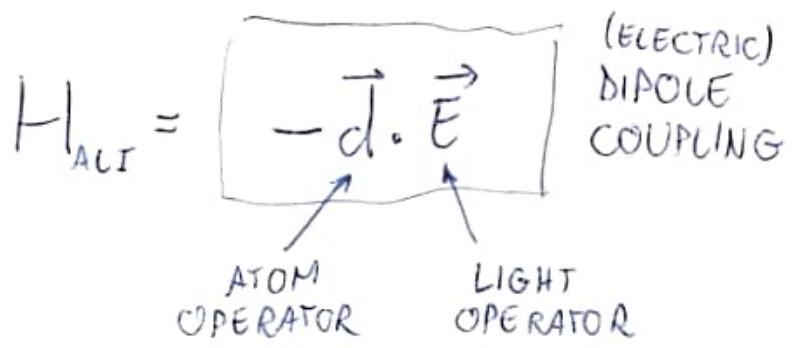
\includegraphics[width=0.5\textwidth]{2025_10_16_22329e0f50bdd2511b17g-13(1)}
\end{center}

FOR AN ALKACI ATOM\\
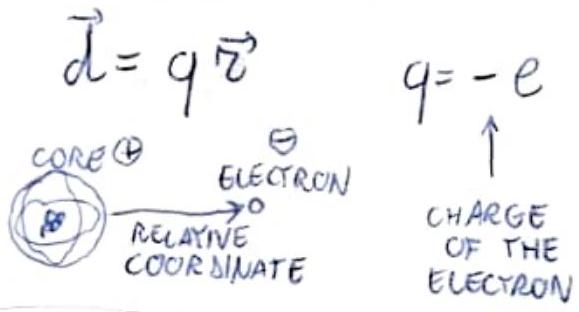
\includegraphics[width=0.5\textwidth, center]{2025_10_16_22329e0f50bdd2511b17g-13(2)}\\
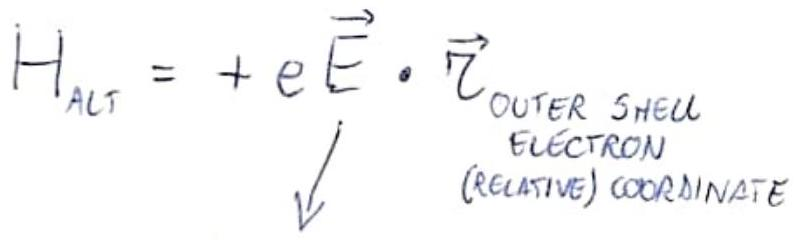
\includegraphics[width=0.5\textwidth, center]{2025_10_16_22329e0f50bdd2511b17g-13}\\
vector in the drectlon of dolarization $\vec{\epsilon}_{K \lambda}$

REFRESHER $\rightarrow$ CLASBICAL DIPOLE\\
$\left.\begin{array}{l}\underset{d}{d}+q \\ \underset{d-q}{d}\end{array}\right\} \begin{gathered}\text { IS a } \triangle P O L E \quad \begin{array}{l}Q+q \\ T a / 2\end{array} \\ \text { THUS }\end{gathered}+\begin{gathered}T-\pi / 2 \\ V-q\end{gathered}$\\
$\hat{I}|q \vec{d}|$ in diefction $+\hat{d}$

We must understand how $\vec{r}$ acts as an operator on ATOMIC LEVELS $\mid N, l, M, \ngtr>$ (electron spin has no el. DI POLE)\\
FACT 1, NO DIAGONAL COMPONENT

$$
\langle n, l, m| \vec{r}|n, l, m\rangle=0
$$

(PRCOF) $\hat{R}$ "PRANTY TRORHATION $\approx \hat{R} \psi(x, y, z)=\psi(-x,-y,-z)$\\
$\tilde{R} \hat{\vec{r}} \tilde{R}^{+}=-r$

$$
\stackrel{s}{R} \psi(r, \theta, \varphi)=\psi(r, \pi-\theta, \varphi+\pi)
$$

$$
\left\{\begin{array}{c}
\mathbb{V} \\
\{\hat{\vec{r}}, \tilde{R}\}=0
\end{array}\right.
$$

$\square \tilde{R}\left(R_{h e}(r) Y_{e_{m}}(\theta, \varphi)\right)=(-1)^{e} R_{n e} Y_{e_{m}}$ WHy?

$$
\begin{aligned}
Y_{e e} & =\sin ^{e}(\theta) e^{i l \varphi} \\
\tilde{R} Y_{e l} & =\sin ^{e}(\pi-\theta) e^{i l(\varphi+\pi)}=e^{i l \pi} e^{i l \varphi} \sin ^{e}(\theta) \\
& =e^{i l \pi} Y_{e l}=(-1)^{e} Y_{e l}
\end{aligned}
$$

$\operatorname{But}_{\text {ALSO }}\left[\tilde{R}, L_{ \pm}\right]=0 \quad[\tilde{R}, \vec{L}]=0 \Leftrightarrow \vec{L}$ WA A

$$
\begin{aligned}
\vec{L}=\vec{r} \times \vec{p} \sim[\tilde{R}, \vec{r} \times \vec{p}] & =\tilde{R} \vec{r} \times \vec{p}-\vec{r} \times \vec{p} \tilde{R} \\
& =(-\vec{r} \tilde{R}) \times \vec{p}-\vec{r} \times(-\tilde{R} \vec{p})=0
\end{aligned}
$$

THEREFORE $\tilde{R} Y_{e-i}(\theta, \varphi)=\frac{1}{\sqrt{e(e+1)-e(e-i)}} \tilde{R} L-Y_{ee}(\theta, \varphi)=$\\
$=\frac{1}{\sqrt{\ldots}} L \cdot \tilde{R} Y_{ee}=\frac{(-1)^{e}}{\sqrt{-}} L-Y_{ee}(\theta, \varphi)=(-1)^{e} Y_{e, l-1}(\theta, \varphi)$

AND BY RECURSION IT WORKS FOR ANY m

BUT NOW CONSIDER

$$
\begin{aligned}
& \langle n, l, m| \vec{r}|n, l, m\rangle=\langle n, l, m| \underbrace{R^{+} R}_{\text {DENTIY }} \vec{r}|n, l, m\rangle= \\
& =-\langle n, l, m| R^{+} \vec{r} R|n, l, m\rangle=-(-1)^{l}\langle n, l m| \vec{r}|n l m\rangle(-1)^{l}= \\
& \text { nons }
\end{aligned}
$$

FACT 2, selection Rule on $l$\\
we start from a (not neoven) equation

$$
\left[L^{2},\left[L^{2}, \vec{r}\right]=2 \hbar^{2}\left\{\vec{r}, L^{2}\right\}\right.
$$

\begin{center}
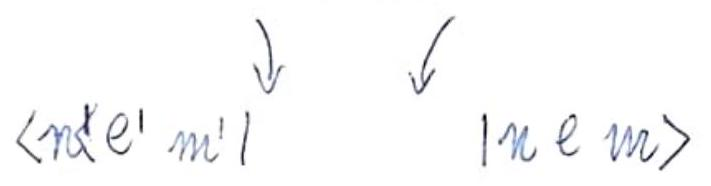
\includegraphics[width=0.5\textwidth]{2025_10_16_22329e0f50bdd2511b17g-14}
\end{center}

THIS CAN BE DEMONSTRATED USING ONCY

$$
\begin{aligned}
& \vec{L}=\vec{r} \times \vec{p} \quad \begin{array}{l}
L^{2}=L_{x}^{2}+L_{y}^{2}+L_{z}^{2} \\
=\vec{L} \cdot \vec{L}
\end{array} \\
& \left\{\tau_{J^{\prime}} p_{T^{\prime}}\right\}=i \hbar \delta_{J^{\prime}} \\
& \text { BUT IT IS SIFFICULT! } \\
& \text { MAYBE AN ASSIGNMENT }
\end{aligned}
$$

$\left\langle n e^{\prime} n n^{\prime}\right|\left(L^{2}\right)^{2} \vec{r}-2 L^{2} r L^{2}+\vec{r}\left(L^{2}\right)^{2}|n e m\rangle=$\\
$2 \hbar^{2}\left\langle n l^{\prime} m^{\prime}\right| \vec{r} L^{2}+L^{2} r|n l m\rangle=$\\
$t^{4}\left(\left[e^{\prime}\left(e^{\prime}+1\right)\right]^{2}-2 e^{\prime}\left(e^{\prime}+1\right) e(e+1)-[e(e+1)]^{2}\right)\left\langle n^{\prime} e^{\prime} m^{\prime}\right| \vec{r}|n e m\rangle=$\\
$2 \hbar^{4}\left(e^{\prime}\left(e^{\prime}+1\right)+e(e+1)\right)\left\langle n^{\prime} e^{\prime} m^{\prime}\right| \vec{r}|n l m\rangle$\\
$O=\left[\left(e^{\prime}\left(e^{\prime}+1\right)-e(e+1)\right)^{2}-2\left(e^{\prime}\left(e^{\prime}+1\right)+e(e+1)\right)\right]\left\langle n^{\prime} e^{\prime} m^{\prime}\right| \vec{r}|n l m\rangle$\\
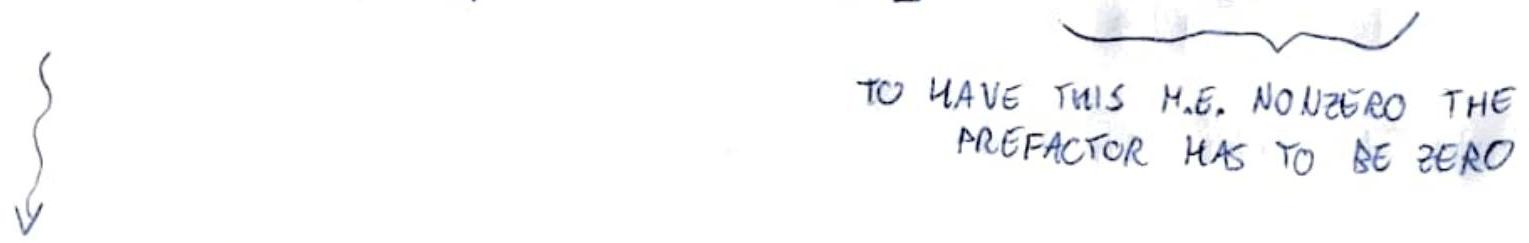
\includegraphics[width=0.5\textwidth, center]{2025_10_16_22329e0f50bdd2511b17g-15}\\
$\underset{\text { (A) }}{\left(e^{\prime}-e+1\right)} \underset{\text { (B) }}{\left(e^{\prime}-e+1\right)} \underset{\text { (C) }}{\left(e+e^{\prime}\right)} \underbrace{\left(e^{\prime}+e+2\right)}_{\text {NEVER ZERO }}$ Wirn $e, e^{\prime} \geqslant 0$

\section*{OPTIONS}
A $\mid e^{\prime}=e+1 \quad \checkmark$ ok\\
B $e^{\prime}=e-1 \quad \checkmark$ ok\\
c $e=e^{\prime}=0$ HOWEVER $\langle n 00| \vec{r}\left|n^{\prime} O 0\right\rangle \quad \begin{gathered}\text { BECAUSE OF PARIYY } \\ \text { ARGUMENT }\end{gathered}$ ARGUMENT\\
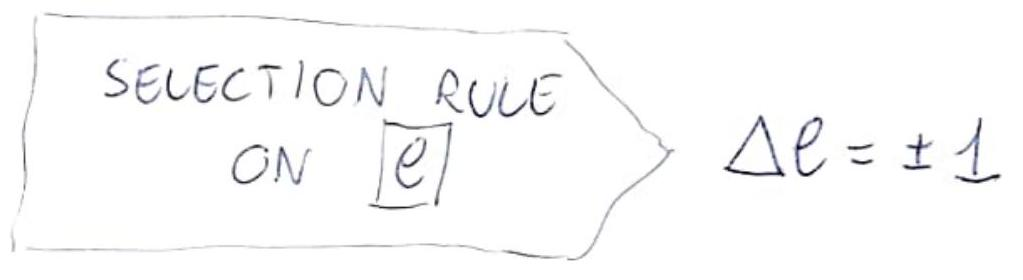
\includegraphics[width=0.5\textwidth, center]{2025_10_16_22329e0f50bdd2511b17g-15(1)}

Fact 3, let's now assume $\vec{E}$ is polarized along $z$-axis\\
$L_{z} \cdot|e, m\rangle=\hbar m$ and $L_{z}=r_{x} p_{y}-r_{y} p_{x}$\\
clearly $\left[L_{z}, z\right]=0$ cuz $z$ commutes with $r_{x, y} p_{x, y}$\\
$0=\left\langle n^{\prime} l^{\prime} m^{\prime}\right|\left[L_{z}, z\right]|n e m\rangle=$\\
$\left\langle n^{\prime} l^{\prime} m^{\prime}\right|\left(L_{z} z \mid-z L_{z}\right)|n l m\rangle=\hbar\left(m^{\prime}-m\right) \underbrace{\left\langle n^{\prime} l^{\prime} m^{\prime}\right| \hat{z}|n l m\rangle}_{\text {TO HAVE THIS MATRA ELEHENT }}$\\
ON M

$$
\Delta m=0
$$

FACT4 NOW $\vec{E}$ POLARIZES ON $\tilde{x}$ (OR $\hat{y}$ ) AXES

$$
\begin{aligned}
& {\left[L_{z}, x\right]=\left(x p_{y}-y p_{x}\right) x-x\left(x p_{y}-y p_{x}\right)=y\left(x p_{x}-p_{x} x\right)=i \hbar y} \\
& {\left[L_{z}, y\right]=\ldots=-i \hbar x}
\end{aligned}
$$

S

$$
\begin{aligned}
& {\left[L_{z}, x+i y\right]=(i \hbar y)+i(-i \hbar x)=\hbar(x+i y) \quad\left[L_{z}, x-i y\right]=-\hbar(x-i y)} \\
& \left\langle n^{\prime} l^{\prime} m^{\prime}\right|\left[L_{z}, x+i y\right]|n e m\rangle=\hbar\left\langle w l^{\prime} m^{\prime}\right|(x+i y)|n e m\rangle
\end{aligned}
$$

$\hbar\left(m^{\prime}-m-1\right)\left\langle n^{\prime} l^{\prime} m^{\prime}\right| x+i y|n l m\rangle=0 \quad$ AND

$$
\hbar\left(m^{\prime}-m+1\right)\left\langle n^{\prime} e^{\prime} m^{\prime}\right| x-i y|n l m\rangle=0
$$

to have $\langle\cdot| x|\cdot\rangle \neq 0$ at least one $\left\langle 0^{\prime}\right| x \pm i y|0\rangle$ hust be nonzero $\rightarrow$

BUT THEN

$$
\begin{aligned}
& m^{\prime}=n+1 \\
& m^{\prime}=m-1
\end{aligned}
$$

Sele ction ROLE ON M xy-plant polarization.

$$
\Delta m= \pm 1
$$

\section*{SODIUM (again)}
\begin{center}
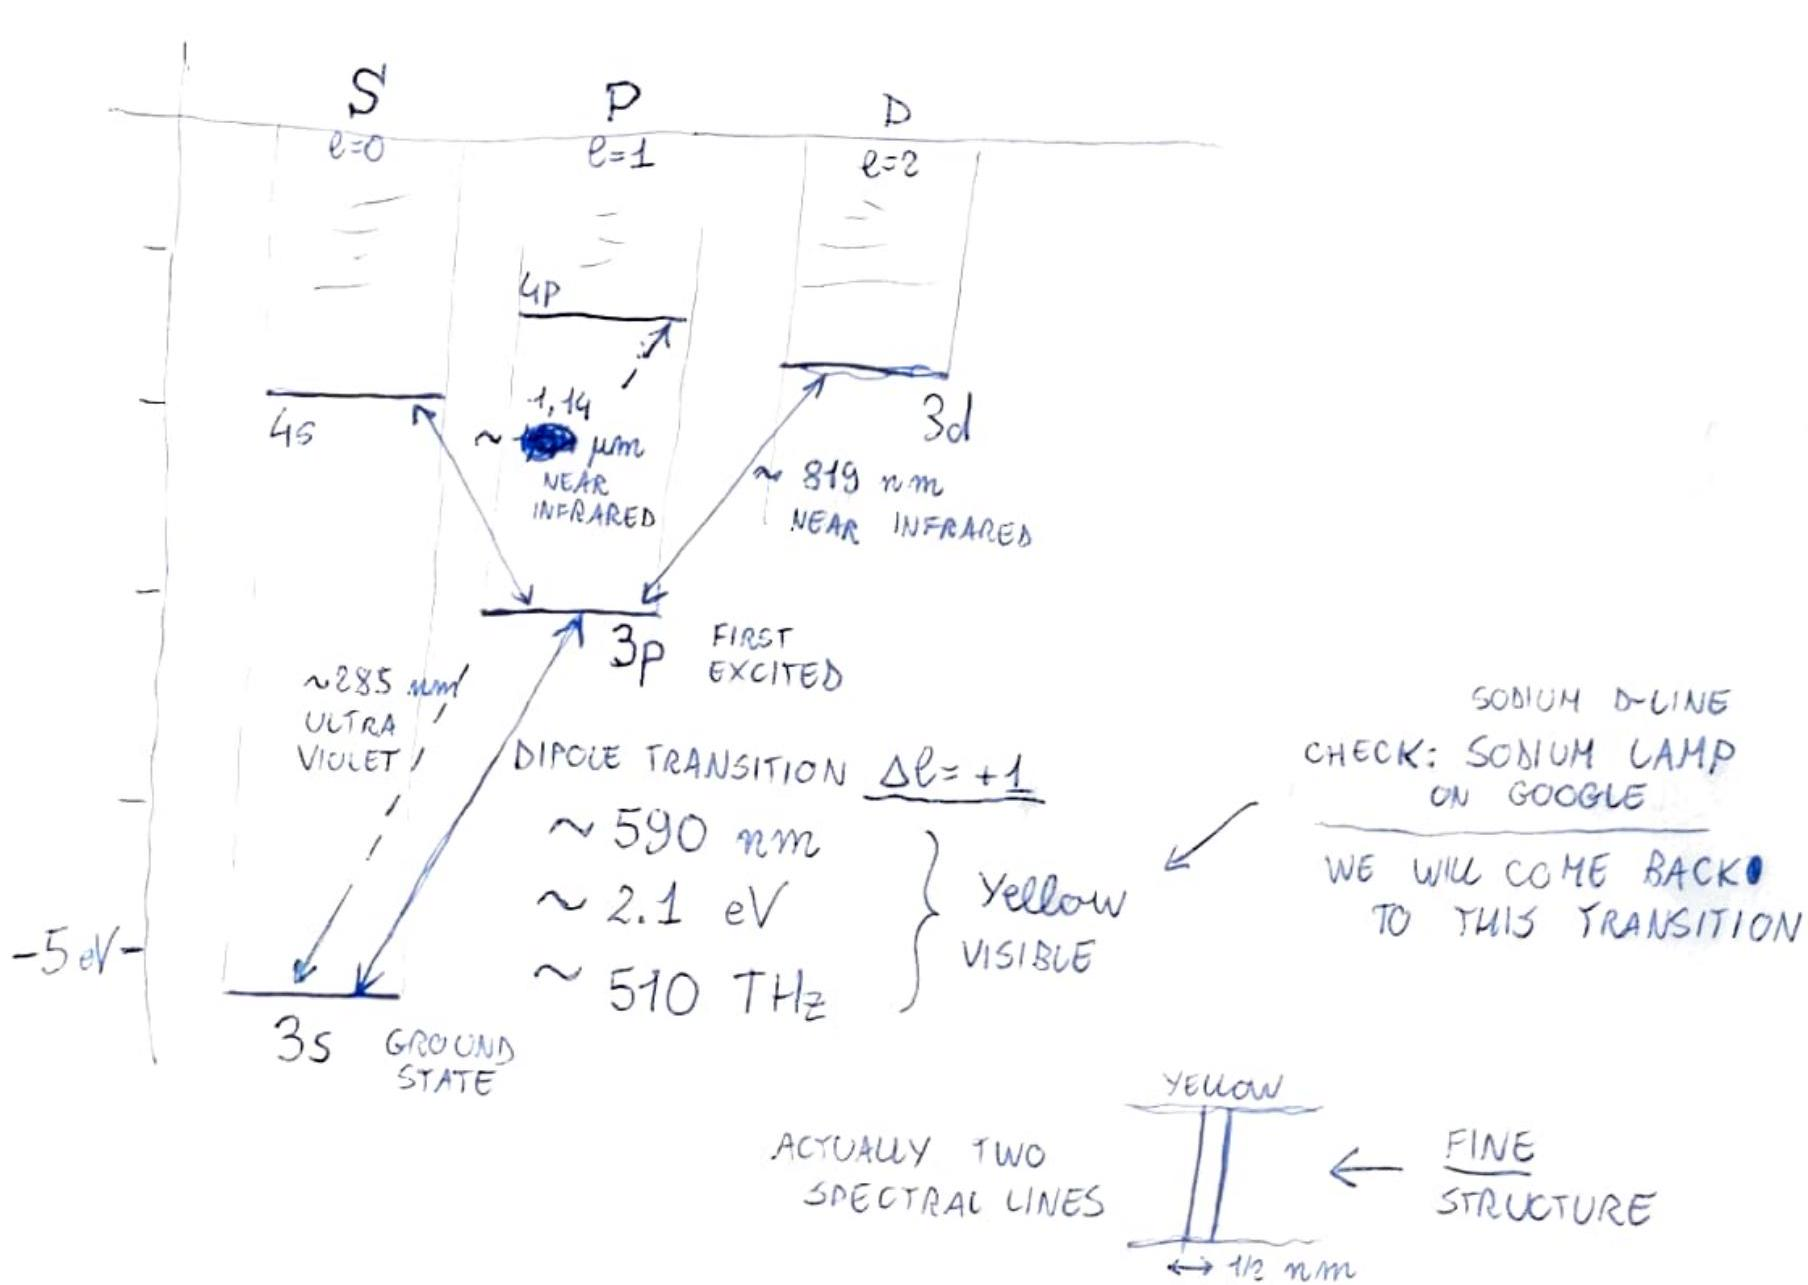
\includegraphics[width=0.5\textwidth]{2025_10_16_22329e0f50bdd2511b17g-16}
\end{center}
